%!TEX root = research_proposal.tex

\chapter{Remaining Work to Complete the Thesis\label{chap:plan}}

In this chapter, we summarize the state of the research and the work that needs to be completed in order to finalize the thesis.
We proceed according to the contributions listed in Section \ref{sec:objective-thesis}.


\section{An aggregate bug  repository for  developers  and  Researchers}

We introduced {\tt BUMPER} (BUg Metarepository for  dEvelopers  and  Researchers),  a  web-based  infrastructure
that  can  be  used  by  software  developers  and  researchers  to access  data  from  diverse  repositories  using  natural  language queries in a transparent manner, regardless of where the data was originally created and hosted.
{\tt BUMPER} have been showcased in the following publications:

\begin{itemize}
	\item Nayrolles, M. \& Hamou-Lhadj, W. BUMPER: A Tool to Cope with Natural Language Search of Millions Bugs and Fixes. In Proceeding of the International Conference on Software Analysis, Evolution, and Reengineering (SANER'16) - Tool Track, pages 649-652, 2016.
	\item Nayrolles, M. \& Hamou-Lhadj, W. BUMPER: Bug Metarepository Search Engine for Developers and Researchers. Consortium for Software Engineering Research Fall, 2015.
\end{itemize}

We consider this contribution to be 100\% complete.

\section{A bug reproduction technique based on a combination of crash traces and model checking.}

In this work, we proposed an approach, called {\tt JCHARMING} (Java CrasH Automatic Reproduction by directed Model checkING) that uses a combination of crash traces and model checking to automatically reproduce bugs that caused field failures.
{\tt JCHARMING} have been showcased in the following publications:

\begin{itemize}
	\item Nayrolles, M. , Hamou-Lhadj, W., Tahar, S. & Larsson, A. (2016). A Bug Reproduction Approach Based on Directed Model Checking and Crash Traces. Journal of Software: Evolution and Process. Wiley. 2016. (Accepted).
	\item Nayrolles, M. , Hamou-Lhadj, W., Tahar, S. & Larsson, A. JCHARMING : A Bug Reproduction Approach Using Crash Traces and Directed Model Checking. In Proceeding of the International Conference on Software Analysis, Evolution, and Reengineering (SANER'15), pages 101-110, 2015. (Best Paper Award).
\end{itemize}

We consider this contribution to be 100\% complete.

\section{An incremental approach for preventing bug and clone insertion at commit time}

We presented {\tt PRECCINT} (PREventing Clones INsertion at Commit Time) and {\tt BIANCA} (Bug Insertion ANticipation by Clone Analysis at merge time) in chapters \ref{chap:clone-detection-pragmatic} and \ref{chap:bianca}.

The efficiency of {\tt PRECCINT} have been accessed.
Early experiments have been conducted for {\tt BIANCA}.
However, we need to conduct additional experiments to measure the efficiency of {\tt BIANCA}.

We consider this contribution to be 40\% complete.

\section{A new taxonomy of bugs based on the location of the correction --- an empirical Study}


In order to classify the research on the different fields related to software maintenance, we can reason about types of bugs at different levels. For
example, we can group bugs based on the developers that fix
them or using information about the bugs such as crash traces.


Our aim is not to improve testing as it is the case in the work of Eldh \cite{Eldh2001} and Hamill et al.\cite{Hamill2014}.
Our objective is to propose a classification that can allow researchers in the filed of mining bug 9 repositiories to use the taxonomy as a new criterion in triaging, prediction, and reproduction of bugs.
By analogy, we can look at the proposed bug taxonomy in a similar way as the clone taxonomy presented by Kapser and Godfrey \cite{CoryKapser}.
The authors proposed seven types of source code clones and then conducted a case study, using their classification, on the file system module of the Linux operating system.
This clone taxonomy continues to be used by researchers to build better approaches for detecting a given clone type and being able to effectively compare approaches with each other.

In this section, we are interested in bugs that share similar fixes.
By a fix, we mean a modification (adding or deleting lines of
code) to an exiting file that is used to solve the bug. With this
in mind, the relationship between bugs and fixes can be
modeled using the UML diagram in Figure \ref{fig:bug-taxo-diag}. The diagram
only includes bugs that are fixed. From this figure, we can
think of four instances of this diagram, which we refer to as
bug taxonomy or simply bug types (see Figure \ref{fig:bug-taxo}).



\begin{figure}[h!]
  \centering
    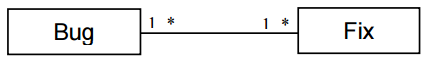
\includegraphics[scale=0.5]{media/bug-taxo-class-diag.png}
    \caption{Class diagram showing the relationship between bugs and fixed
    \label{fig:bug-taxo-diag}}
\end{figure}

\begin{figure}[h!]
  \centering
    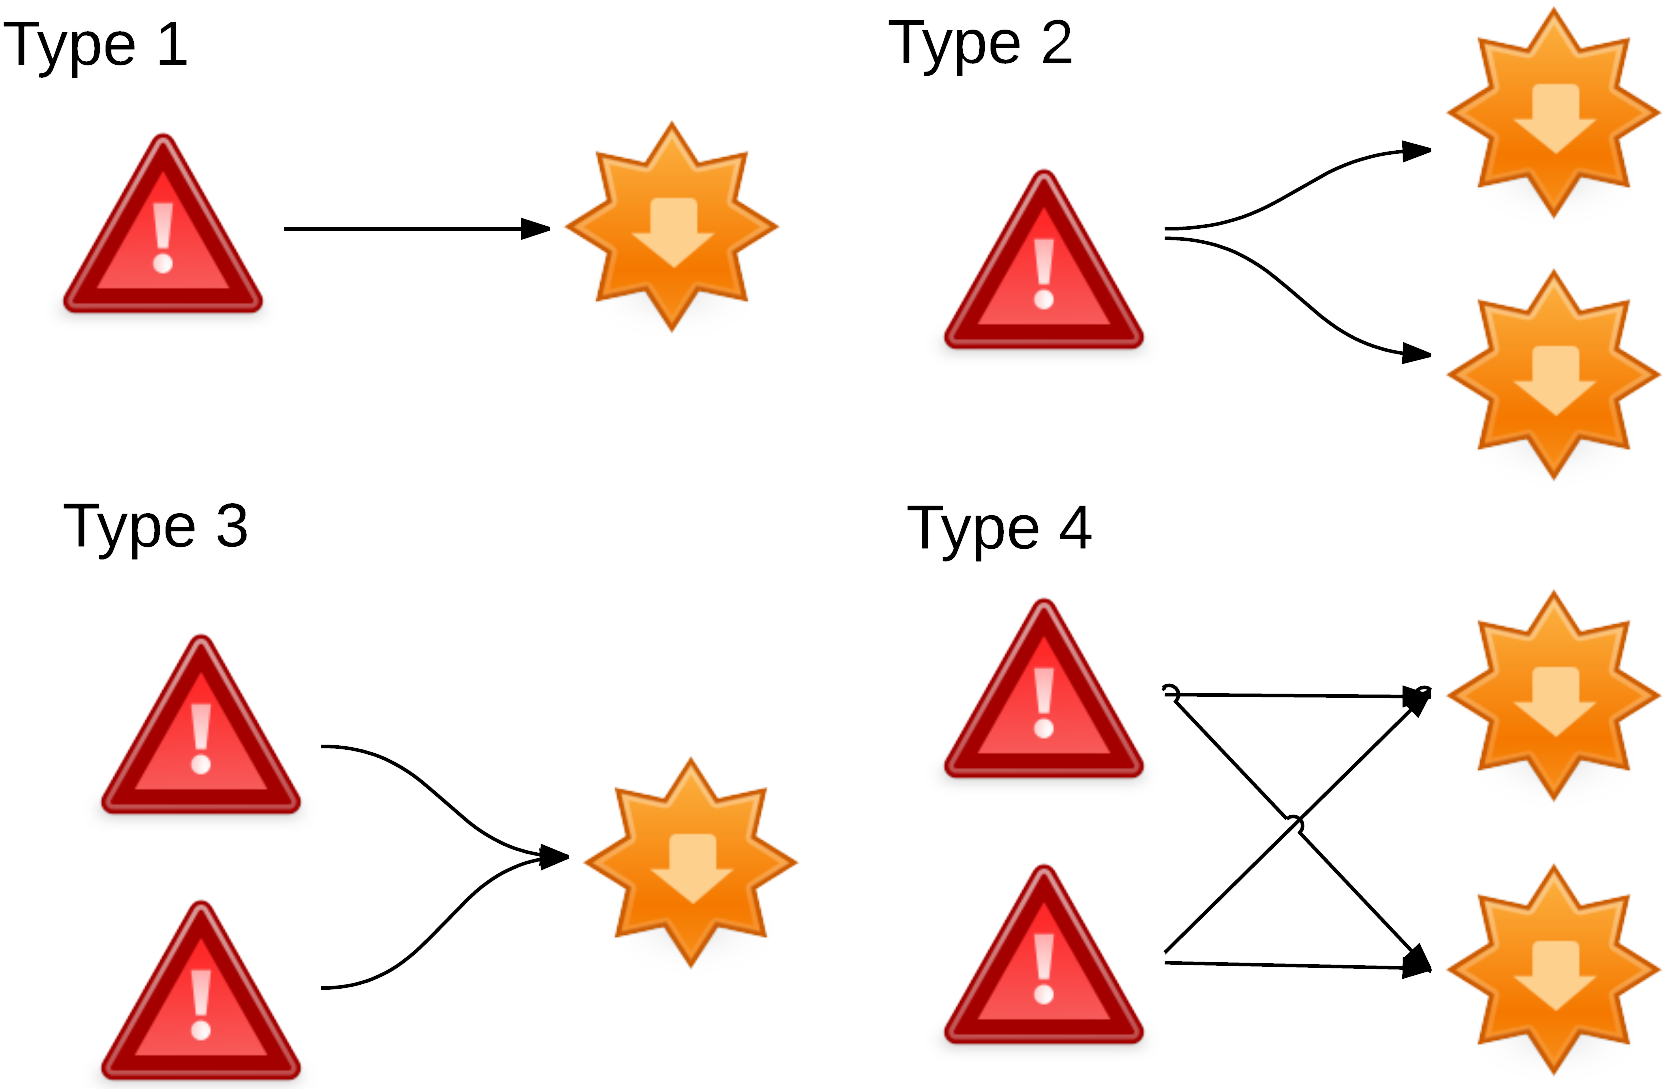
\includegraphics[scale=0.8]{media/bug-taxo.png}
    \caption{Proposed Taxonomy of Bugs
    \label{fig:bug-taxo}}
\end{figure}


The first and second types are the ones we intuitively know
about. Type 1 refers to a bug being fixed in one single location
(i.e., one file), while Type 2 refers to bugs being fixed in more
than one location. In Figure 2, only two locations are shown
for the sake of clarity, but many more locations could be
involved in the fix of a bug. Type 3 refers to multiple bugs that
are fixed in the exact same location. Type 4 is an extension of
Type 3, where multiple bugs are resolved by modifying the
same set of locations. Note that Type 3 and Type 4 bugs are
not duplicates, they may occur when different features of the
system fail due to the same root causes (faults).
We conjecture that knowing the proportions of each type
of bugs in a system may provide insight into the quality of the
system. Knowing, for example, that in a given system the
proportion of Type 2 and 4 bugs is high may be an indication
of poor system quality since many fixes are needed to address
these bugs. In addition, the existence of a high number of
Types 3 and 4 bugs calls for techniques that can effectively
find bug reports related to an incoming bug during triaging.
This is similar to the many studies that exist on detection of
duplicates (e.g., \cite{Runeson2007,Sun2010,Nguyen2012}), except that we are not looking for
duplicates but for related bugs (bugs that are due to failures of
different features of the system, caused by the same faults). To
our knowledge, there is no study that exmpirically examines
bug data with these types in mind, which is the main objective
of this section. More particularly, we are interested in the
following research questions:

\begin{itemize}
	\item RQ1: What are the proportions of different types of bugs?
	\item RQ2: How complex is each type of bugs?
	\item RQ3: How fast are these types of bugs fixed?
\end{itemize}


\subsection{Study Setup}

Figure \ref{fig:bug-taxo-flow} illustrates our data collection and analysis
process that we present here and discuss in more detail in the
following subsections. First, we extract the raw data from the
two bug report management systems used in this study
(Bugzilla and Jira). Second, we extract the fix to the bugs
from the source code version control system of Netbeans and
Apache (Maven and Git).

\begin{figure}[h!]
  \centering
    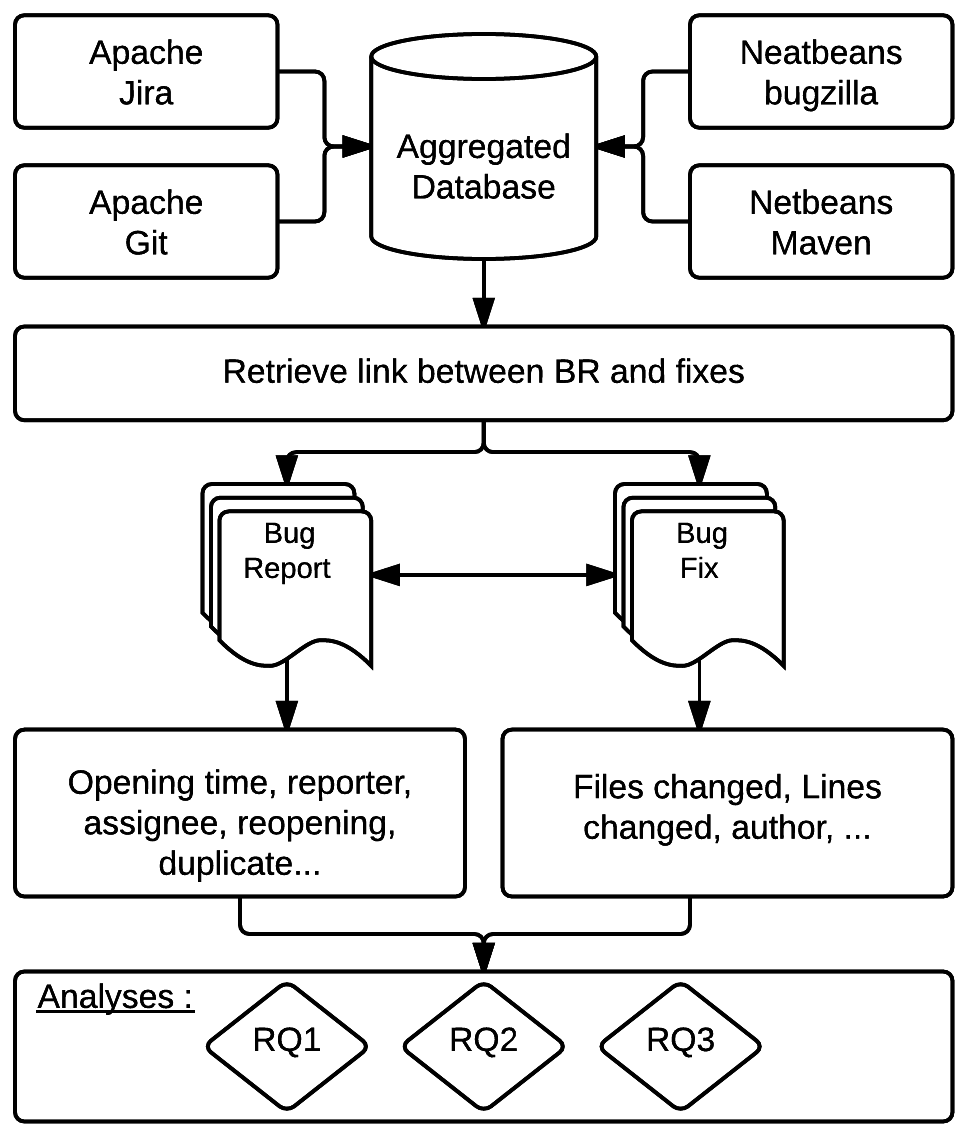
\includegraphics{media/bug-taxo-flow.png}
    \caption{Data collection and analysis process of the study
    \label{fig:bug-taxo-flow}}
\end{figure}


The extracted data is
consolidated in one database where we associate each bug
report to its fix. We mine relevant characteristics of BRs and
their fixes such as opening time, number of comments,
number of times the BR is reopened, number of changesets
for BR and the number of files changed and lines modified
for fixes or patch. Finally, we analyse these characteristics to
answer the aforementioned research questions (RQ).

We consider this contribution to be 50\% complete.

\section{Publication Plan\label{sec:publication-plan}}

This section presents our current and planned publications.
Publications 1 to 5 have already been accepted in various international conferences and journals.

\begin{itemize}
	\item {\bf Publication 1}. A Bug Reproduction Approach Using Crash Traces and Directed Model Checking. In Proceeding of the International Conference on Software Analysis, Evolution, and reengineering (SANER'15), pages 101-110, 2015. (Best Paper Award).
	\item {\bf Publication 2}. An Empirical Study on the Handling of Crash Reports in a Large Software Company: An Experience Report. In Proceeding of the IEEE International Conference on Software Maintenance and Evolution (ICSME'15), pages 342-351, 2015. (Third author)
	\item {\bf Publication 3}. BUMPER: Bug Metarepository Search Engine for Developers and Researchers. Consortium for Software Engineering Research Fall (CSER'15), 2015.
	\item {\bf Publication 4}. BUMPER: A Tool to Cope with Natural Language Search of Millions Bugs and Fixes. In Proceeding of the International Conference on Software Analysis, Evolution, and Reengineering (SANER'16) -  pages 649-652, 2016.
	\item {\bf Publication 5}.  A Bug Reproduction Approach Based on Directed Model Checking and Crash Traces. Journal of Software: Evolution and Process. Wiley. 2016. (in press).
	\item {\bf Publication 6}. A New Taxonomy of Bugs Based on the Location of the Correction: An Empirical Study (submitted to IEEE Transaction on Software Engineering).
	\item {\bf Publication 7}. JAPPA: An Automatic Patch Generation Approach Using Model Checking and Changesets History will be submitted to the Empirical Software Engineering Journal (EMSE) special issue on Automatic Software Repair.
	\item {\bf Publication 8}. PRECINCT: An Incremental Approach for Preventing Clone Insertion at Commit Time will be submitted to the Journal of Systems and Software.
	\item {\bf Publication 9}. BIANCA: Bug Insertion ANticipation by Clone Analysis at commit-time will be submitted to IEEE Software special issue on Theme Issue on Reliability Engineering for Software.
	\item {\bf Publication 10}. RESEMBLE: REcommendation System based on cochangE Mining at Block LEvel will be submitted to SANER'17.
	\item {\bf Publication 11}. Software Maintenance at Commit-Time will be submitted to IEEE Software.
	\item {\bf Thesis}.  Ph.D. thesis.
\end{itemize}

Table \ref{tab:pubPlan} presents an overview of the publication plan.
For each contribution, the title, the target conference or journal and the time at which we plan to work on it is given.
The red line represents the current time.

\begin{table}[]
\centering
\small
\caption{Publications Plan}
\label{tab:pubPlan}
\begin{tabular}{p{7cm}llllllllllll}
Title & Target & &  &  &  &  &  &  &  &  &  &  \\ \hline \hline
\multicolumn{13}{c}{2014} \\ \hline
 &  & J & F & M & A & M & J & J & A & O & N & D \\ \hline
Courses Requirements & n.a & \cellcolor{green!25} & \cellcolor{green!25} & \cellcolor{green!25} & \cellcolor{green!25} & \cellcolor{green!25} & \cellcolor{green!25} & \cellcolor{green!25} &  &  &  &  \\ \hline
Literature Review & n.a &  &  &  & \cellcolor{green!25} & \cellcolor{green!25} & \cellcolor{green!25} & \cellcolor{green!25} &  &  &  &  \\ \hline
A Bug Reproduction Approach Using Crash Traces and Directed Model Checking & SANER &  &  &  &  &  &  &  & \cellcolor{green!25} & \cellcolor{green!25} & \cellcolor{green!25} & \cellcolor{green!25} \\ \hline \hline
\multicolumn{13}{c}{2015} \\ \hline
 &  & J & F & M & A & M & J & J & A & O & N & D \\ \hline
An Empirical Study on the Handling of Crash Reports in a Large Software Company: An Experience Report. & ICSME & \cellcolor{green!25} & \cellcolor{green!25} & \cellcolor{green!25} &  &  &  &  &  &  &  &  \\ \hline
BUMPER: Bug Metarepository Search Engine for Developers and Researchers. & CSER &  &  &  & \cellcolor{green!25} & \cellcolor{green!25} & \cellcolor{green!25} & \cellcolor{green!25} & \cellcolor{green!25} & \cellcolor{green!25} & \cellcolor{green!25} & \cellcolor{green!25} \\ \hline
BUMPER: A Tool to Cope with Natural Language Search of Millions Bugs and Fixes. & SANER &  &  &  & \cellcolor{green!25} & \cellcolor{green!25} & \cellcolor{green!25} & \cellcolor{green!25} & \cellcolor{green!25} & \cellcolor{green!25} & \cellcolor{green!25} & \cellcolor{green!25} \\ \hline
A Bug Reproduction Approach Based on Directed Model Checking and Crash Traces. & JSEP &  &  &  & \cellcolor{green!25} & \cellcolor{green!25} & \cellcolor{green!25} & \cellcolor{green!25} & \cellcolor{green!25} & \cellcolor{green!25} & \cellcolor{green!25} & \cellcolor{green!25} \\ \hline \hline
\multicolumn{13}{c}{2016} \\ \hline
 &  & J & F & M & A & M & J & J & A & O & N & D \\ \hline
A New Taxonomy of Bugs Based on the Location of the Correction: An Empirical Study & TSE & \cellcolor{green!25} & \cellcolor{green!25} & \cellcolor{green!25} & \cellcolor{green!25} & \multicolumn{1}{c!{\color{red}\vrule}}{\cellcolor{green!25}} &  &  &  &  &  &  \\ \hline
Preparing the Ph.D research proposal & n.a & \cellcolor{green!25} & \cellcolor{green!25} & \cellcolor{green!25} & \cellcolor{green!25} & \multicolumn{1}{c!{\color{red}\vrule}}{\cellcolor{green!25}} &  &  &  &  &  &  \\ \hline
JAPPA: An Automatic Patch Generation Approach Using Model Checking and Changesets History & EMSE &  &  &  &  & \multicolumn{1}{c!{\color{red}\vrule}}{\cellcolor{green!25}} & \cellcolor{green!25} & \cellcolor{green!25} & \cellcolor{green!25} &  &  &  \\ \hline
PRECINCT: An Incremental Approach for Preventing Clone Insertion at Commit Time & JSS &  &  &  &  & \multicolumn{1}{c!{\color{red}\vrule}}{\cellcolor{green!25}} & \cellcolor{green!25} & \cellcolor{green!25} & \cellcolor{green!25} &  &  &  \\ \hline
Bug Insertion ANticipation by Clone Analysis at commit-time & IEEE SW &  &  &  &  & \multicolumn{1}{c!{\color{red}\vrule}}{} &  &  &  & \cellcolor{green!25} & \cellcolor{green!25} & \cellcolor{green!25} \\ \hline \hline
\multicolumn{13}{c}{2017}  \\ \hline
 &  & J & F & M & A & M & J & J & A & O & N & D \\ \hline
 RESEMBLE: REcommendation System based on cochangE Mining at Block LEvel & SANER & \cellcolor{green!25} & \cellcolor{green!25}  & \cellcolor{green!25} & \cellcolor{green!25} &  &  &  &  &  &  &  \\ \hline
Software Maintenance at Commit-Time & IEEE SW & \cellcolor{green!25} & \cellcolor{green!25}  & \cellcolor{green!25} & \cellcolor{green!25} &  &  &  &  &  &  &  \\ \hline
Write the Ph.D Thesis & n.a &  &  &  &  &  \cellcolor{green!25} & \cellcolor{green!25} & \cellcolor{green!25} & \cellcolor{green!25} &  &  &
\end{tabular}
\end{table}
